\documentclass{examen}

\begin{document}
\modulo{Lenguajes de marcas}

\pregunta{Modifica el HTML llamado Ejercicio 1 para que quede como la figura 1.
Ten en cuenta que:
\begin{itemize}
\item{Puedes modificar el HTML y a�adir lo que quieras. Si lo haces recuerda entregar
la hoja con el HTML modificado.}
\item{Puedes escribir el CSS que quieras. No hace falta intentar optimizar el tama�o.}
\item{Los titulares est�n centrados, tienen un fondo gris y un tipo de letra de un tama�o grande.}
\item{Siempre que se ve CSS o HTML el tipo de letra es Arial Black, cursiva y negrita.}
\item{La tabla tiene un borde pero no las celdas individuales. El texto dentro de las celdas va centrado.}
\item{El punto 2 de la lista va subrayado. Tambi�n lo est� el primer punto de la lista de abajo.}
\end{itemize}
}{3.5}
\break
\begin{figure}[h]
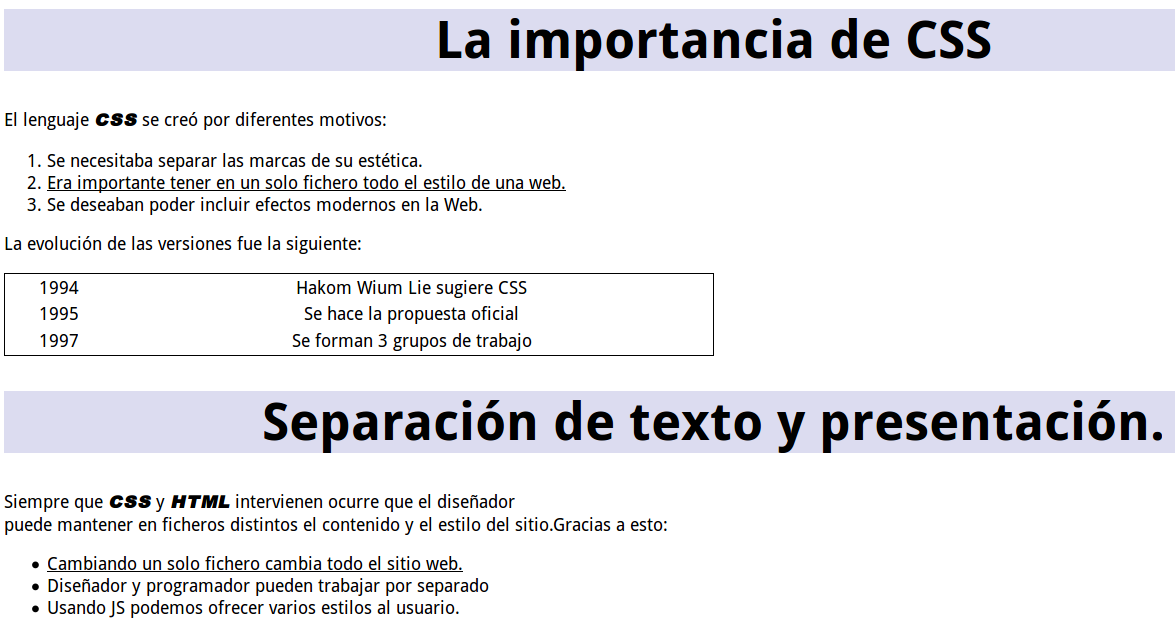
\includegraphics[scale=0.4]{examen-img/ej_css.png} 
\caption{Ejercicio 1}
\end{figure}

\break

\pregunta{Dado el HTML llamado Ejercicio 2, crea el CSS asociado para que la p�gina quede tal y como se muestra en la figura 2. Ten en cuenta que puedes modificar el HTML a�adiendo los atributos {\tt id} y {\tt class} que necesites. Ten en cuenta que:
\begin{itemize}
\item{La cabecera y el pie son de color gris y tienen borde.}
\item{La cabecera tiene una fuente diferente (elige la que quieras).}
\item{Se ha cambiado la posici�n normal de muchas cajas.}
\item{La caja del pie de p�gina no se mueve aunque el usuario se mueva hacia arriba o hacia abajo. Adem�s tiene una anchura del 25\%.}
\end{itemize}
}{3.5}
\begin{figure}[h]
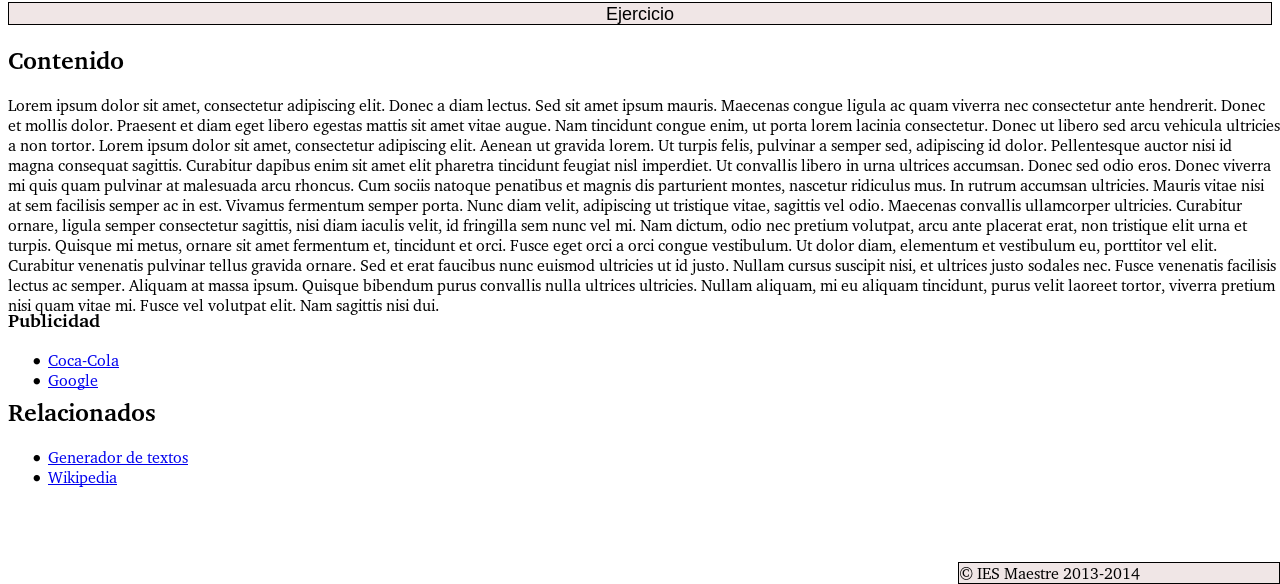
\includegraphics[scale=0.3]{examen-img/ej2.png} 
\caption{Ejercicio 2}
\end{figure}

\break

\pregunta{Dado el HTML llamado Ejercicio 3, crea el CSS asociado para que la p�gina quede tal y como se muestra en la figura 3. Ten en cuenta que puedes modificar el HTML a�adiendo los atributos {\tt id} y {\tt class} que necesites. Ten en cuenta que:
\begin{itemize}
\item{La cabecera, los elementos relacionados y la publicidad ocupan un ancho de un 25\%.}
\item{La caja que contiene el texto no tiene bordes. Observa bien que el texto de dicha caja fluye alrededor de otras cajas.}
\end{itemize}
}{3.5}
\break
\begin{figure}[h]
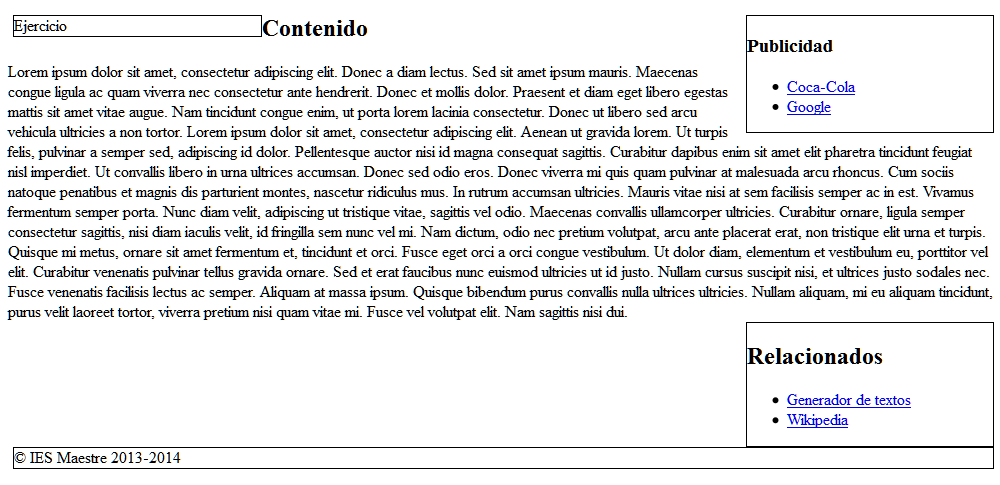
\includegraphics[scale=0.4]{examen-img/ej3.png} 
\caption{Ejercicio 3}
\end{figure}


\break

\begin{verbatim}
                Ejercicio 1
                
<h1>La importancia de CSS</h1>
<p>El lenguaje CSS se cre� por diferentes motivos:</p>
<ol>
    <li>Se necesitaba separar las marcas de su est�tica.</li>
    <li>Era importante tener en un solo fichero todo el estilo de una web.</li>
    <li>Se deseaban poder incluir efectos modernos en la Web.</li>
</ol>
<p>La evoluci�n de las versiones fue la siguiente:</p>
<table>
    <tbody>
        <tr><td>1994</td><td>Hakom Wium Lie sugiere CSS</td></tr>
        <tr><td>1995</td><td>Se hace la propuesta oficial</td></tr>
        <tr><td>1997</td><td>Se forman 3 grupos de trabajo</td></tr>
    </tbody>
</table>
<h1>Separaci�n de texto y presentaci�n.</h1>
<p>Siempre que CSS y HTML intervienen ocurre que el dise�ador puede mantener
en ficheros distintos el contenido y el estilo del sitio.Gracias a esto:</p>
<ul>
    <li>Cambiando un solo fichero cambia todo el sitio web.</li>
    <li>Dise�ador y programador pueden trabajar por separado</li>
    <li>Usando JS podemos ofrecer varios estilos al usuario.</li>
    
</ul>
\end{verbatim}



\break

\begin{verbatim}
              Ejercicio 2
              
<div>
    <div>
        <h3>Publicidad</h3>
        <ul>
            <li><a href="http://coca-cola.es">Coca-Cola</a></li>
            <li><a href="http://google.es">Google</a></li>
        </ul>
        
    </div>
    <div>
        <h2>Contenido</h2>
        Lorem ipsum ...
    </div>
    <div>
        <h2>Relacionados</h2>
        <ul>
            <li>
                <a href="http://es.lipsum.com/">Generador de textos</a>
            </li>
            <li>
                <a href="http://es.wikipedia.org">Wikipedia</a>
            </li>
        </ul>
    </div>
</div>
<footer>
    &copy; IES Maestre 2013-2014
</footer>

</body>
</html>

\end{verbatim}


\break

\begin{verbatim}
                 Ejercicio 3
<header>
    Ejercicio 3
</header>
<div>
    <div>
        <h3>Publicidad</h3>
        <ul>
            <li><a href="http://coca-cola.es">Coca-Cola</a></li>
            <li><a href="http://google.es">Google</a></li>
        </ul>
        
    </div>
    <div>
        <h2>Contenido</h2>
        Lorem ipsum ...
    </div>
    <div>
        <h2>Relacionados</h2>
        <ul>
            <li>
                <a href="http://es.lipsum.com/">Generador de textos</a>
            </li>
            <li>
                <a href="http://es.wikipedia.org">Wikipedia</a>
            </li>
        </ul>
    </div>
</div>
<footer>
    &copy; IES Maestre 2013-2014
</footer>

</body>
</html>

\end{verbatim}

\end{document}
